\documentclass[landscape,paperwidth=43truein,paperheight=33.1truein,fontscale=0.3]{baposter}
\usepackage{graphics}
\usepackage{color}
\usepackage{multicol}
\usepackage{amsmath}
\usepackage{amssymb, wasysym}

\begin{document}
\definecolor{myfavoritecolor}{rgb}{0.0 2.55 0}

\begin{poster}
{%Keyword=value pairs
  % Color style
  bgColorOne=white,
  bgColorTwo=white,
  borderColor=black,
  headerColorOne=black,
  headerColorTwo=blue,
  headerFontColor=white,
  boxColorOne=white,
  boxColorTwo=myfavoritecolor,
  % Format of textbox
  textborder=roundedleft,
  % Format of text header
  eyecatcher=true,
  headerborder=closed,
  headerheight=0.15\textheight,
  headershape=roundedright,
  headershade=shadelr,
  boxshade=plain,
  headerfont=\Large\textrm,
}
{%Eyecatcher
   \resizebox{!}{.2\textheight}{
\includegraphics{transparent_solar_physics_logo.png}}
}
{%Poster Title
   {Identifying Extra Spectral Content In MOSES Images Using Cross Correlation}
}
{%Author
   Jake Parker and Charles C.\ Kankelborg\\
   \textit{Physics Department, Montana State University, Bozeman, MT 59717}\\
   jacob.parker3@montana.edu\\
   
}
{%Logo
   \resizebox{!}{.13\textheight}{
\includegraphics{msuvertcmyk.pdf}}
}

%%%%%%%%%%%%%%%%%%%%%%%%%%%%%%%%%%%%
%         Zeroth Column            %
%%%%%%%%%%%%%%%%%%%%%%%%%%%%%%%%%%%%

\headerbox{Abstract}{name=abstract,column=0}{
\par

\footnotesize{The \textit{MOSES} (\textit{Multi-Order Solar EUV Spectrograph})  sounding rocket was launched February 8th, 2006 to capture images of the sun at 304 \AA. The \textit{MOSES} concave grating forms solar images in multiple spectral orders, in an effort to measure line profiles from a single exposure over a wide field of view. We present a preliminary identification of spectral content in \textit{MOSES} images. The cross correlation of subtracted images provide evidence of spectral content besides the normal 304 \AA \ He II line. We place confidence on the peaks in correlation by cross correlating random data that is statistically representative of \textit{MOSES} data. These significant peaks indicate a contribution to intensity from several coronal lines.  These lines are individually weak, but if not taken into account, they would significantly increase the residuals when inverting \textit{MOSES} images to obtain spectra.z
}


}


\headerbox{Instrument Concept}{name=concept ,span=1,below=abstract}{

\
		\begin{center}
		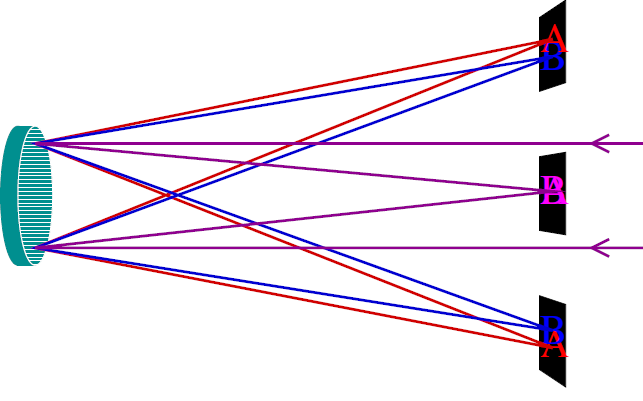
\includegraphics[scale=.25]{instrument.png}
	\end{center}			
	
	\
	
The \textit{MOSES} optics consist of a concave grating, secondary fold flat mirror, and three Charged Couple Device \textit{(CCD)} detectors. Incident light on the grating is diffracted onto the \textit{CCD}'s in the -1, 0, and +1 spectral orders. Each order contains different combination of spectral and spacial information. [2]



}

\headerbox{Significance Testing}{name=signif,span=1,below=concept ,above=bottom}{

	

\resizebox{1\columnwidth}{!}{\includegraphics{sigtest_5_cropped.png}}
Here is the cross correlation of our two \textit{MOSES} subtracted images (in blue) and significance levels (red).  We tested the significance of the peaks by correlating random data generated from \textit{MOSES} columns.
}









%%%%%%%%%%%%%%%%%%%%%%%%%%%%%%%%%%%%
%          First Column            %
%%%%%%%%%%%%%%%%%%%%%%%%%%%%%%%%%%%%

\headerbox{MOSES Images}{name=Images,column=1,span=3}{
\begin{center}
\begin{tabular}{lll}
  \begin{minipage}{.315\columnwidth}
    \resizebox{1\columnwidth}{!}{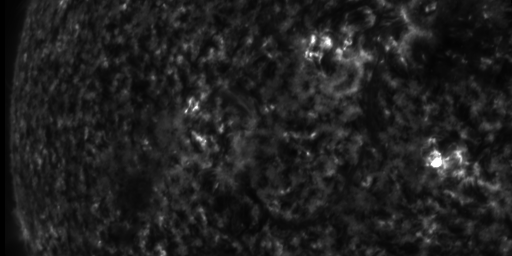
\includegraphics{../../../../../IDL/mcor/Outputs/super_zero.png}}
    \footnotesize{Time Integrated Zero Order}  
 \end{minipage}&
 \begin{minipage}{.315\columnwidth}
    \resizebox{1\columnwidth}{!}{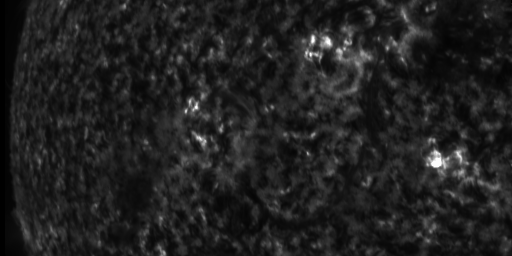
\includegraphics{../../../../../IDL/mcor/Outputs/super_plus.png}}
    \footnotesize{Time Integrated Plus Order}  
 \end{minipage}&
\begin{minipage}{.315\columnwidth}
    \resizebox{1\columnwidth}{!}{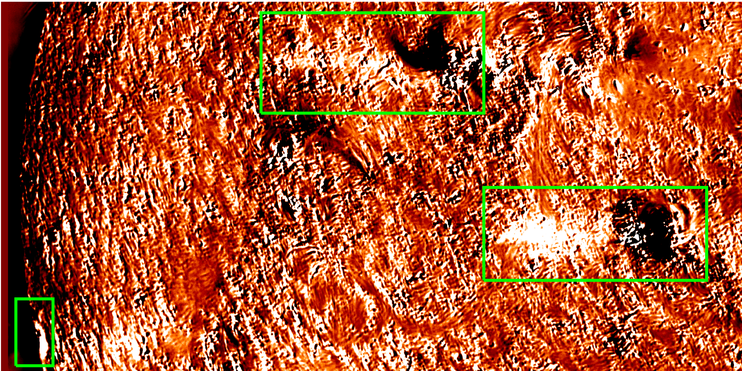
\includegraphics{../../../../../IDL/mcor/Outputs/super_pz.png}}
    \footnotesize{Zero Order Image Subtracted From Plus Order Image}  

\end{minipage}
\end{tabular}
\end{center}
Pictured here are the zero and plus order \textit{MOSES} images, as well as an image of the zero order subtracted for the plus order.  The plus and zero order images have been aligned to maximize the cross correlation in the grating dispersion (horizontal) direction as well as averaged over all exposures.  The subtracted image highlights the subtle differences between the two images.  These differences are caused by objects differing in wavelength from the dominant (He II 304 \AA) wavelength. Small differences are caused by differing point spread functions between orders and Doppler shifted material. Large differences, boxed in green, are indicative of extra spectral content. That content is identified by cross correlating subtracted images in the dispersion direction.
}

\headerbox{Forward Model}{name=for,column=1,span=2,below=Images,above=bottom}{
\begin{tabular}{c c c}
  \begin{minipage}{.35\columnwidth}
	\footnotesize{Modelled Subtracted Image}    
	\end{minipage}&
	\begin{minipage}{.25\columnwidth}
	\footnotesize{Quality of Fit}    
	\end{minipage}&
	\begin{minipage}{.25\columnwidth}
	\footnotesize{Spectral Content}    
	\end{minipage}
	\\
	\begin{minipage}{.35\columnwidth}
	\resizebox{1\columnwidth}{!}{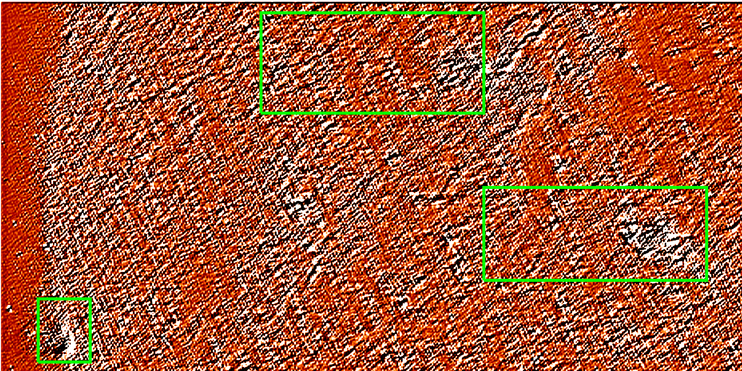
\includegraphics{../../../../../IDL/mcor/Outputs/eit_ch_max_pz.png}}
	\end{minipage}&
	\begin{minipage}{.25\columnwidth}
	\resizebox{1\columnwidth}{!}{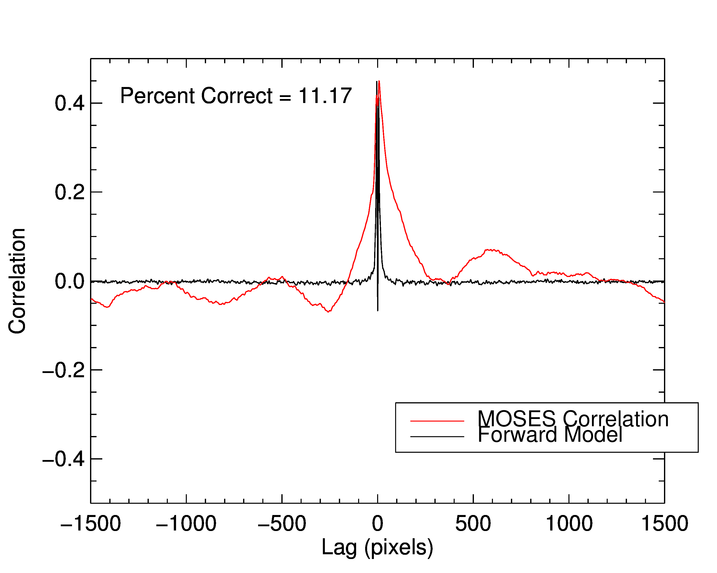
\includegraphics{../../../../../IDL/mcor/Outputs/eit_ch_max_fit.png}}  
	\end{minipage}&
	\begin{minipage}{.25\columnwidth}
	\resizebox{1\columnwidth}{!}{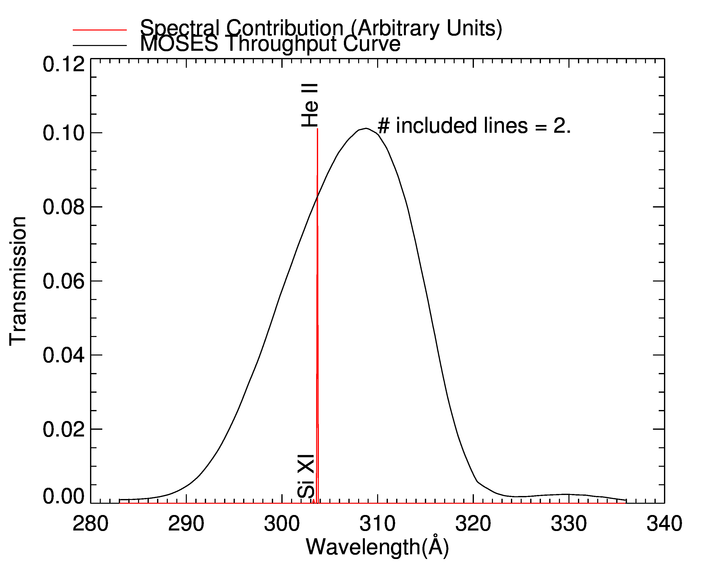
\includegraphics{../../../../../IDL/mcor/Outputs/eit_ch_max_spec.png}}  
	\end{minipage}
	\\
	\begin{minipage}{.35\columnwidth}
	\resizebox{1\columnwidth}{!}{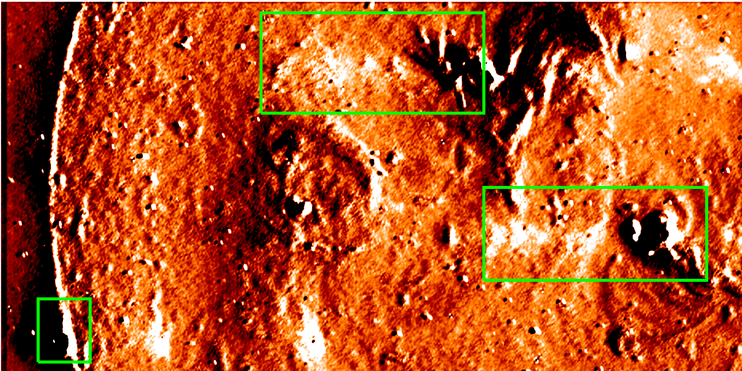
\includegraphics{../../../../../IDL/mcor/Outputs/eit_ch_5_pz.png}}
	\end{minipage}&
	\begin{minipage}{.25\columnwidth}
    \resizebox{1\columnwidth}{!}{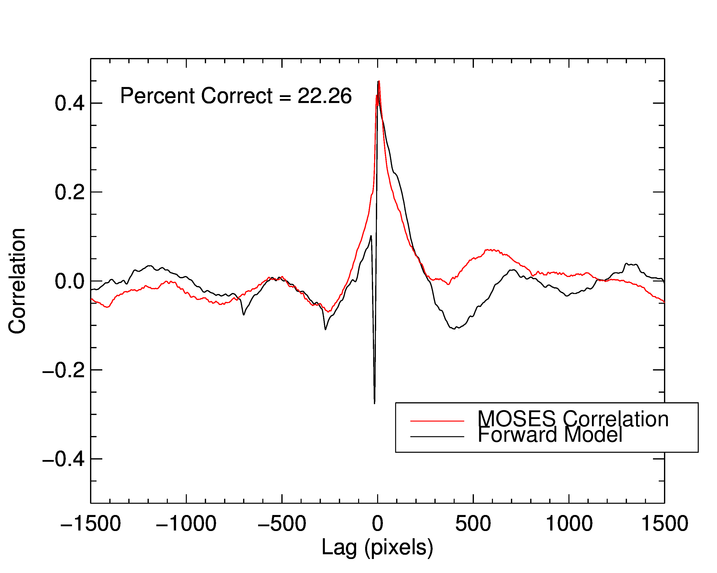
\includegraphics{../../../../../IDL/mcor/Outputs/eit_ch_5_fit.png}}
	\end{minipage}&
	\begin{minipage}{.25\columnwidth}
    \resizebox{1\columnwidth}{!}{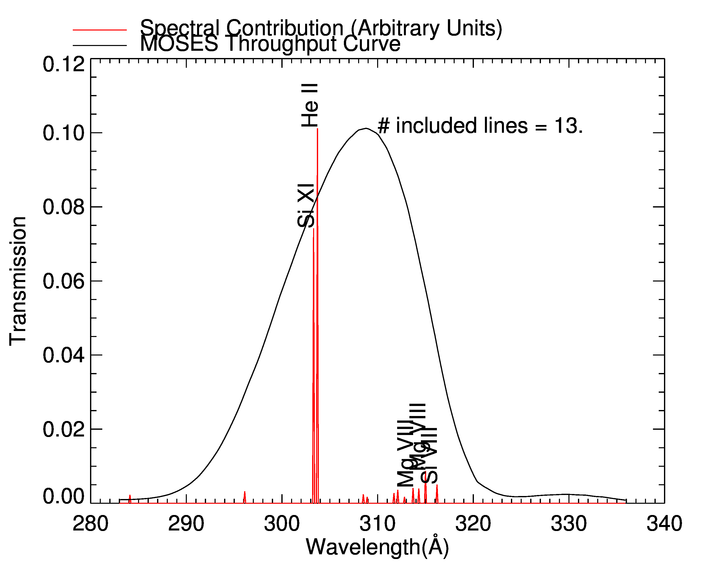
\includegraphics{../../../../../IDL/mcor/Outputs/eit_ch_5_spec.png}}
	\end{minipage}
	\\
	\begin{minipage}{.35\columnwidth}
    \resizebox{1\columnwidth}{!}{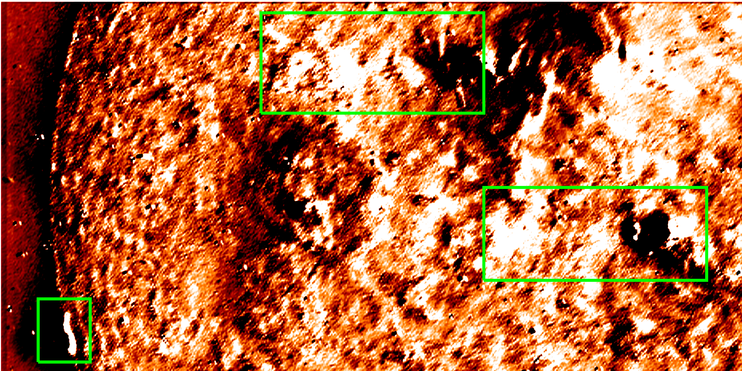
\includegraphics{../../../../../IDL/mcor/Outputs/eit_ch_1_pz.png}}
	\end{minipage}&
	\begin{minipage}{.25\columnwidth}
    \resizebox{1\columnwidth}{!}{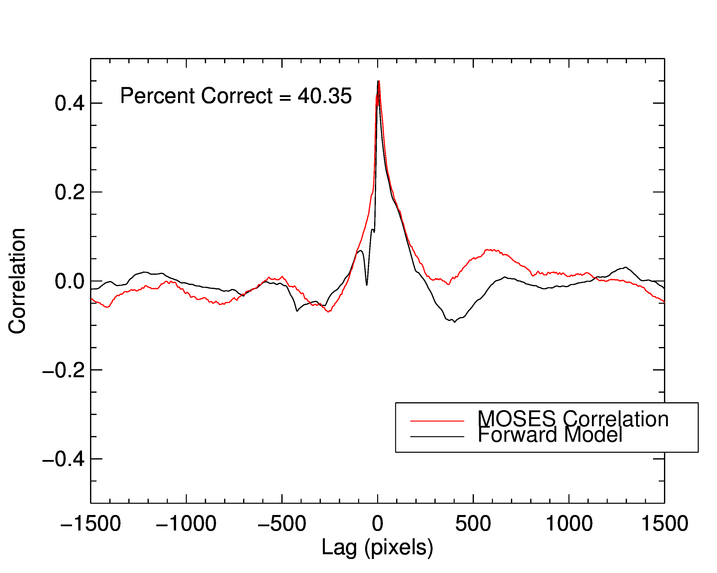
\includegraphics{../../../../../IDL/mcor/Outputs/eit_ch_1_fit.png}}
	\end{minipage}&
	\begin{minipage}{.25\columnwidth}
    \resizebox{1\columnwidth}{!}{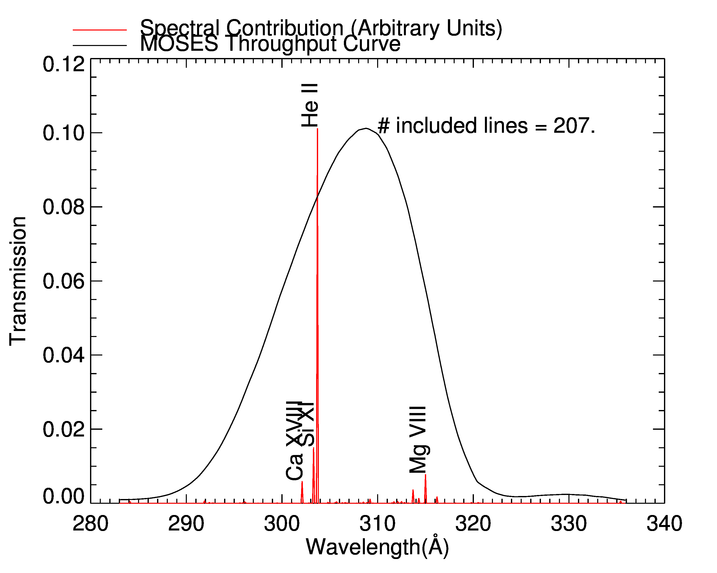
\includegraphics{../../../../../IDL/mcor/Outputs/eit_ch_1_spec.png}}
	\end{minipage}
	\end{tabular}
    
     

Our forward model generates \textit{MOSES} subtracted images using EIT images and Chianti synthetic spectrum.  For each line in the spectral cube we use an average of EIT images that is the closest proxy in temperature. Including lower intensity lines and different combinations of Chianti DEMs, as well as increased levels of He II, improves our fit to the \textit{MOSES} correlation function. [0,1]

}

%%%%%%%%%%%%%%%%%%%%%%%%%%%%%%%%%%%%
%          Second Column           %
%%%%%%%%%%%%%%%%%%%%%%%%%%%%%%%%%%%%






%%%%%%%%%%%%%%%%%%%%%%%%%%%%%%%%%%%%
%          Third Column            %
%%%%%%%%%%%%%%%%%%%%%%%%%%%%%%%%%%%%
\headerbox{Best Fit Chianti DEM}{name=spec,column=3,span=1,below=Images}{
\begin{center}
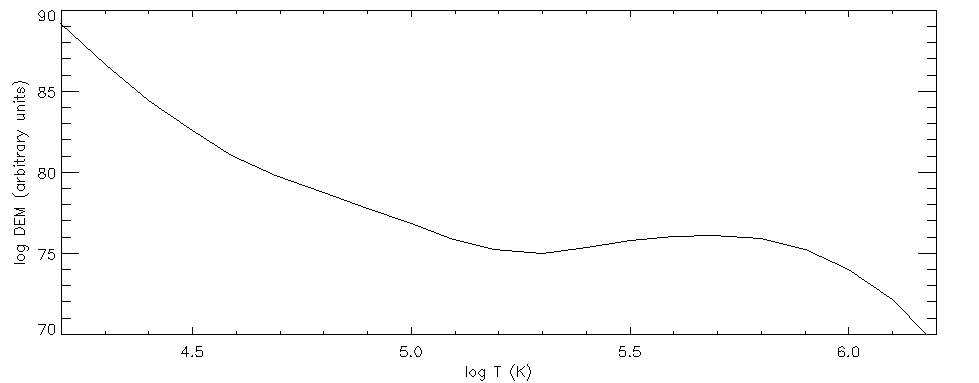
\includegraphics[scale=.2]{../../../../../IDL/mcor/Outputs/bestfitdem.png}

\end{center}

}

\headerbox{Conclusion}{name=con,column=3,below=spec}{ \footnotesize{
Our best fit model shows a coronal contribution to \textit{MOSES} images of about 30\% , one third of which is from Si XI.  We will account for this extra content when examining the residuals of future inversions. This fit also included 20\% more He II than was accounted for in Chianti DEMs.  Our future experiment, the \textit{EUV Snapshot Imaging Spectrograph}, will have an improved optical layout to deal with the contamination from these faint lines. 
}
}

\headerbox{Acknowledgment}{name=ack,column=3,below=con}{ 
\tiny{
This work is partially supported by the NASA Heliophysics Sounding Rocket Program, grant NNX14AK71G.
}

}
\headerbox{References}{name=refs,column=3,below=ack,above=bottom}{
\begin{minipage}{\columnwidth}
\tiny{[0]Dere et al., 1997,Landi et al., 2012; ApJS, 744, 99}

\tiny{[1]	Delaboudinière, J.-P. et al.,1995}

\tiny{[2] Fox et al., 2010}

\end{minipage}
  

}


\end{poster}
\end{document}